\section{Experiments}
	We conduct various experiments to evaluate the effectiveness of \modelname{} on two datasets: KDDCUP  and XuetangX.\footnote{All datasets and codes used in this paper is publicly available at \url{http://www.moocdata.cn}.}
	%both KDDCUP dataset and XuetangX dataset.
	
\subsection{Experimental Setup} 
%	\subsubsection{Implementation Details.}
	\subsubsection{Implementation Details.}We implement \modelname{} with TensorFlow  
	and adopt Adam \cite{kingma2014adam} to optimize the model. To avoid overfitting, we apply $L_2$ regularization on the weight matrices. We adopt Rectified Linear Unit (Relu)~\cite{nair2010rectified} as the activation function. All the features are normalized before fed into \modelname{}. We test \modelname{}'s performance on both KDDCUP  and XuetangX datasets. For the KDDCUP dataset, the history period and prediction period are set to 30 days and 10 days respectively by the competition organizers. We do not use the attention mechanism of \modelname{} on this data, as there is no context information provided in the dataset. For the XuetangX dataset, the history period is set to 35 days, prediction period is set to 10 days, i.e., $D_h=35, D_p=10$.
	
    
	\subsubsection{Comparison Methods.}
	We conduct the comparison experiments for following methods:
	\begin{itemize}
		\item{\textbf{LR}}: logistic regression model.
		\item{\textbf{SVM}}: The support vector machine with linear kernel.
		\item{\textbf{RF}}: Random Forest model.
		\item{\textbf{GBDT}}: Gradient Boosting Decision Tree.
		\item{\textbf{DNN}}: $3$-layer deep neural network.
	    \item{\textbf{\modelname{}}}: The \modelname{} model.
		%\item{\textbf{CFIN-attn}}: AFIN model without using attention mechanism. The activity feature map is fed into DNN layer directly.
		%\item{\textbf{CFIN-ctx}}: AFIN model without context smoothing for activity features. 
		\item{\textbf{\modelname{}-en}}: The assembled \modelname{} using the strategy proposed in Model Ensemble.
\end{itemize}	

	For baseline models (LR, SVM, RF, GBDT, DNN) above, we use all the features (including learning activity $\mathbf{X}$ and context information $\mathbf{Z}$) as input. 
	When training the models,  we tune the parameters based on 5-fold cross validation (CV) with the grid search, and use the best group of parameters in all experiments. The evaluation metrics include Area Under the ROC Curve (AUC) and F1 Score (F1).
	
	\subsection{Prediction performance}
	
	\begin{table}
		\centering
		\caption{Overall Results on KDDCUP dataset and IPM courses of XuetangX  dataset. }
		\setlength{\tabcolsep}{2.3mm}\begin{tabular}{c|cc|cc}
			\hline \hline
			              &\multicolumn{2}{c|}{KDDCUP} &\multicolumn{2}{c}{XuetangX}\\
			  Methods & AUC (\%) & F1 (\%) & AUC (\%) & F1 (\%) \\

			 \hline
			  LRC                      & 86.78 & 90.86   &82.23  & 89.35 \\
			  %\hline 
			  %LRC-Aug              & 87.21 &91.47     &     84.01        &  90.19          \\
			  \hline
		     SVM                   &  88.56	  & 91.65	   &   82.86  &89.78 \\
			%\hline
			%SVM-Aug           &      &       &   83.97        &   90.18         \\
			\hline
			RF                       & 88.82  & 91.73  &83.11  &89.96 \\
			%\hline
			%RF-Aug               & 88.96  & 92.14  &84.15  &90.26 \\
			\hline
			DNN                   &  88.94     & 91.81           & 85.64  &90.40 \\
			\hline
			GBDT        & 89.12& 91.88 & 85.18& 90.48\\
			%\hline
			%GBDT-Aug & 89.82 & 92.73 &86.12 &90.81 \\
			 %AFIN-attn           &   89.92 &92.01& 82.82&  91.98\\
			 %\hline
			 %AFIN-ctx       &    88.31 & 91.54 & 82.15& 91.83\\
			 \hline
			 \modelname{}					&90.07 &92.27   & 86.40& 90.92\\
			\hline
			\modelname{}-en         & \textbf{90.93}    &\textbf{92.87} &  \textbf{86.71}   & \textbf{90.95} \\
			\hline	\hline
		\end{tabular}
		\label{tab:allRes}
	\end{table}


	Table \ref{tab:allRes} presents the results on KDDCUP dataset and IPM courses of XuetangX dataset for all comparison methods. Overall, \modelname{}-en gets the best performance on both two datasets, and its AUC score on KDDCUP dataset achieves 90.93\%, which is comparable to the winning team of KDDCUP 2015$^2$.
	%\footnote{https://biendata.com/competition/kddcup2015/rank/}. \modelname{} also beats the other baseline methods. 
	Compared to LR and SVM, \modelname{} achieves 1.51 -- 3.29\% and 3.54 -- 4.17\% AUC score improvements on KDDCUP  and XuetangX, respectively. Moreover, compared to the ensemble methods (i.e. RF and GBDT) and DNN, \modelname{} also shows a better performance. 
 %Moreover, by comparing the performance of \textbf{-attn}, \textbf{AFIN-ctx} and \textbf{AFIN}, we find that both context information and attention mechanism can enhance the prediction performance of \textbf{AFIN}. In particular, the context-smoothing can improve $1.76\%$ AUC score on KDDCUP dataset.

 %\subsection{Attention Analysis}
 %By analyzing attention scores across different cluster of users, we can identify contribution of each feature for different kinds of users. Table \ref{tab:AttnWeight} shows the average attention weights of different clusters in \ref{}. 
  	\begin{figure*}
  	\centering
  	\subfigure[Strategy 1: Certificate driven]{
  		\centering
  		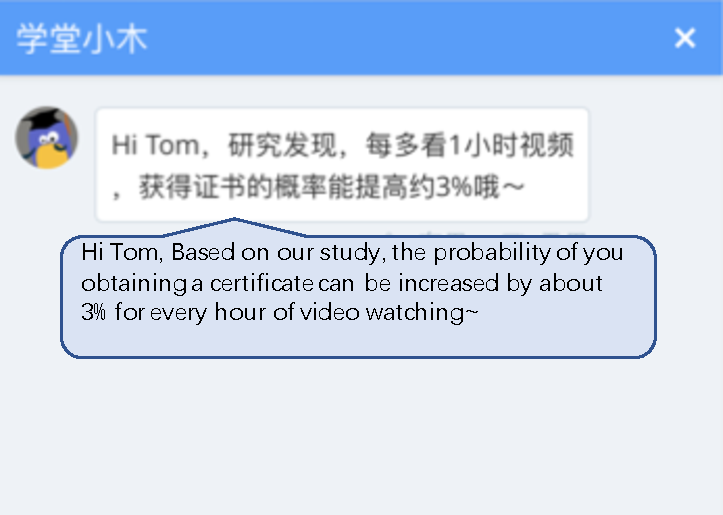
\includegraphics[height=3.7cm]{snapshot_1.pdf}
  	}
  	\subfigure[Strategy 2: Certificate driven in video]{
  		\centering
  		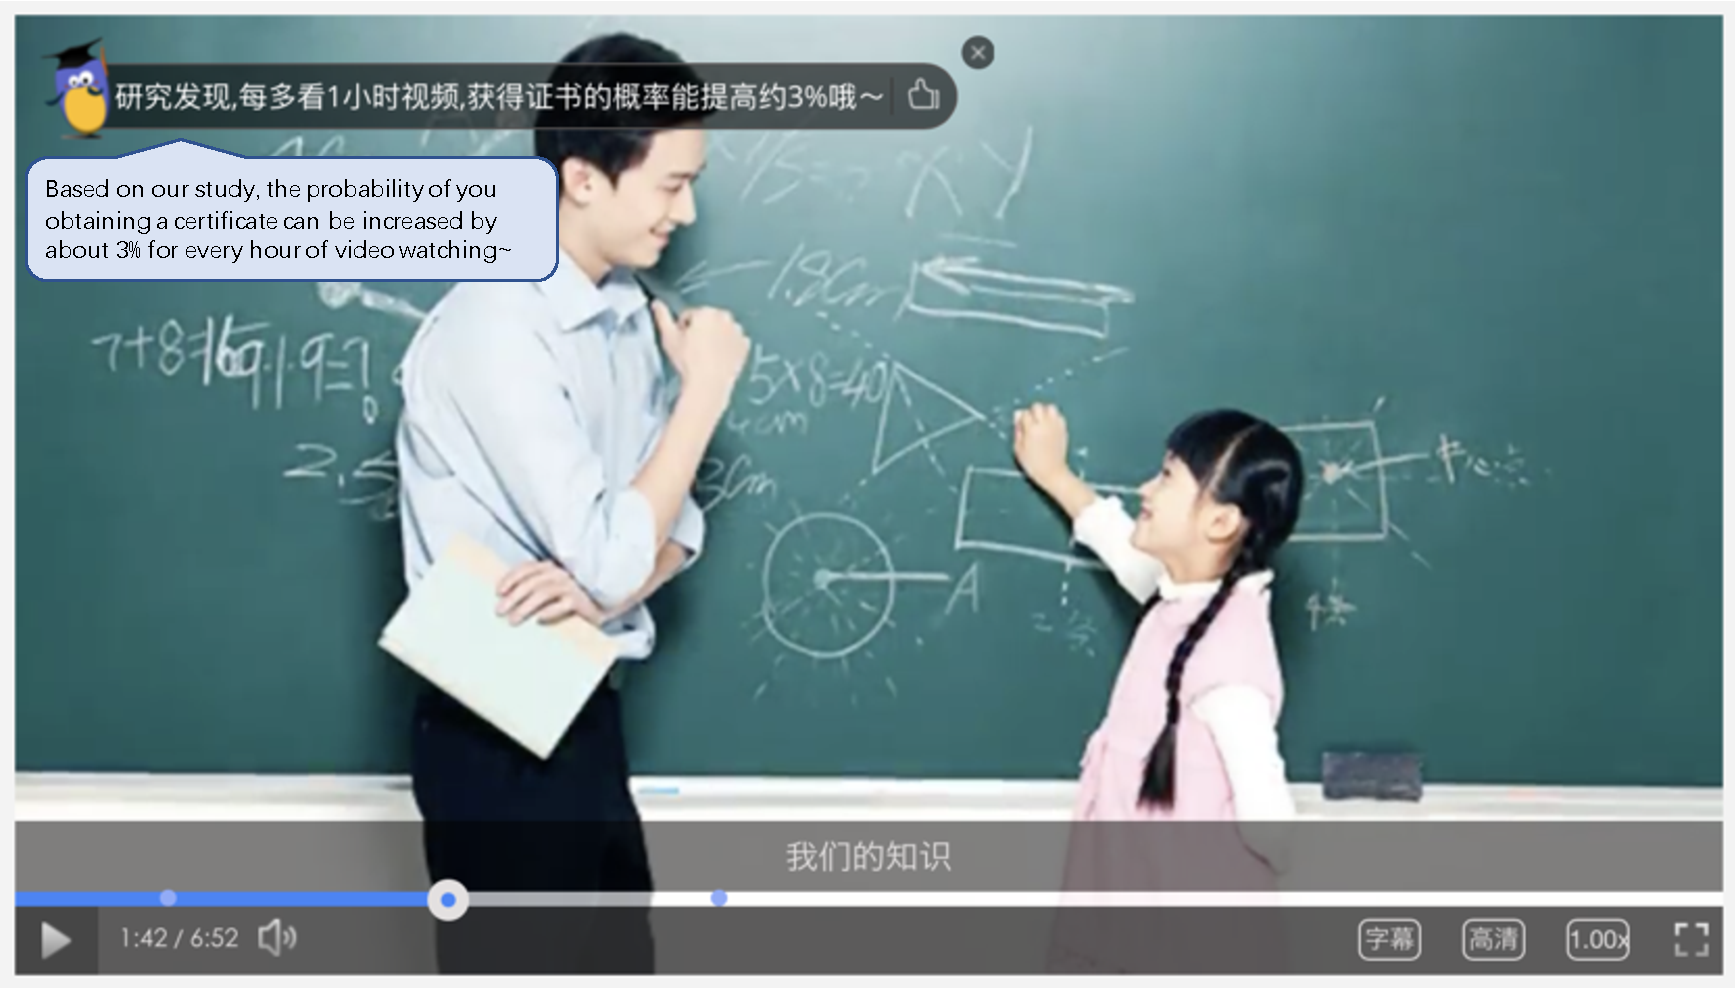
\includegraphics[height=3.7cm]{snapshot_2.pdf}
  	}
  	\subfigure[Strategy 3: Effort driven]{
  		\centering
  		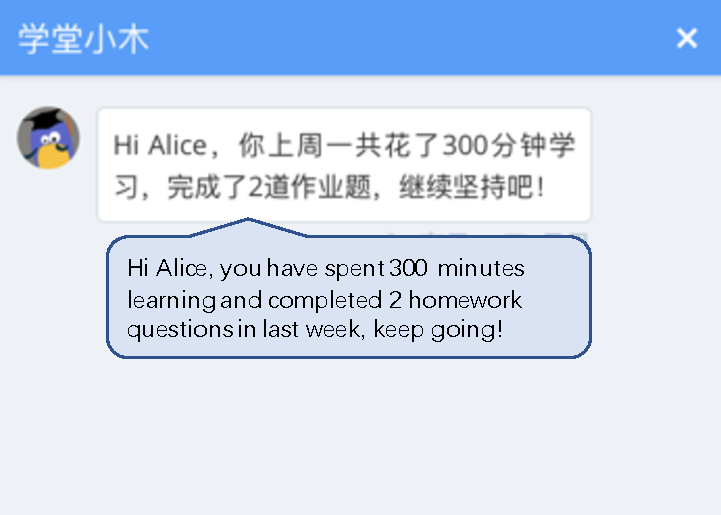
\includegraphics[height=3.7cm]{snapshot_new.pdf}
  	}
  	\caption{Snapshots of the three intervention strategies.} 
  	\label{fig:snapshot}
  \end{figure*}
  
  
  \subsection{Feature Contribution}
  	\begin{table}
		\caption{Contribution analysis for different engagements on KDDCUP dataset and IPM courses of XuetangX dataset.}
		\centering
		\setlength{\tabcolsep}{1.2mm}\begin{tabular}{lcccc}
		\hline \hline
			              & \multicolumn{2}{c}{KDDCUP} & \multicolumn{2}{c}{XuetangX} \\
			{Features}                &AUC (\%)   & F1 (\%)  & AUC (\%)   & F1 (\%)  \\ \hline 
			{All}                     & 90.07 & 92.27 & 86.50 & 90.95     \\ \hline
	   	  - Video         &  87.40 & 91.61     &84.40	  &90.32 \\ 
	      - Forum         & 88.61 & 91.93    & 85.13  &  90.41 \\
		  - Assignment   & 86.68  & 91.39     & 84.83  & 90.34 \\
		  %- (Video + Forum)       &  84.70 & 91.4      &84.42   & 90.31  \\
		  %- (Video + Assignment)   & 84.32& 91.17      &  83.14     &  89.63  \\
		  %- (Forum + Assignment)    & 85.07 &   91.49  &  84.72      & 90.29    \\
			 \hline \hline
 \end{tabular}

	  \label{tab:featImp}	
	\end{table}
	
	\begin{table}
    	\centering
    	\caption{Average attention weights of different clusters. C1-C5 --- Cluster 1 to 5; CAR --- average correct answer ratio. }
    	\small
    	\label{tab:AttnWeight}
    	\setlength{\tabcolsep}{1.8mm}\begin{tabular}{@{}c@{}|l@{}|c|c|c|c|c@{}}
    		\hline
    		\hline
    		Category &  Type   & C1& C2 & C3& C4&C5 \\
    		\hline
    		\multirow{3}{*}{video}&  \#watch &0.078 &0.060 &0.079&0.074 & 0.072\\	
    		\cline{2-7}
    		& \#stop     &0.090 & 0.055 & 0.092&0.092& 0.053\\
    		\cline{2-7}
    		& \#jump   &0.114 & 0.133 & 0.099&0.120& 0.125\\
    		\hline
    		\multirow{2}{*}{forum}&  \#question & 0.136 & 0.127 &0.138 & 0.139 & 0.129 \\
    		\cline{2-7}
    		& \#answer &0.142 &0.173&0.142&0.146&0.131\\
    		\hline
    		\multirow{2}{*}{assignment} & CAR &0.036 & 0.071 & 0.049& 0.049 & 0.122\\
    		\cline{2-7}
    		& \#reset  &0.159 & 0.157& 0.159& 0.125& 0.136\\
    		\hline
    		\multirow{2}{*}{session}    & seconds &0.146 &0.147& 0.138& 0.159& 0.151\\
    		\cline{2-7}                
    		&  count     &0.098 &0.075& 0.103&0.097& 0.081\\ 
    		\hline	
    		\hline
    	\end{tabular}
    	\normalsize
    \end{table}  
	
 	 In order to identify the importance of different kinds of engagement activities in this task, we conduct feature ablation experiments for three major activity features, i.e., video activity, assignment activity and forum activity, on two datasets. Specifically, we first input all the features to the \modelname{}, then remove every type of activity features one by one to watch the variety of performance. The results are shown in Table \ref{tab:featImp}. We can observe that all the three kinds of engagements are useful in this task. On KDDCUP, assignment plays the most important role, while on XuetangX, video seems more useful. 
 	 %Furthermore, the performance decrease rapidly when we remove the video activity and assignment activity together on XuetangX dataset.
 	 
 	 We also perform a fine-grained analysis for different features on different groups of users. Specifically, we feed a set of typical features into \modelname{}, and compute their average attention weights for each cluster. The results are shown in Table \ref{tab:AttnWeight}. We can observe that the distributions of attention weights on the five clusters are quite different. The most significant difference appears in CAR (correct answer ratio): Its attention weight on cluster 5 (hard workers) is much higher than those on other clusters, which indicates that correct answer ratio is most important in predicting dropout for hard workers. While for users with more forum activities (cluster 2), answering questions in forum seems to be the key factor, as the corresponding attention weight on ``\#question'' is the highest. Another interesting thing is about the users with high dropout rates (cluster 1, 3 and 4). They get much higher attention wights on the number of stopping video and watching video compared to cluster 2 and cluster 5. This indicates that the video activities play an more important role in predicting dropout for learners with poor engagements than active learners.
 	 
 	\hide{
	\subsection{Discussion for SPM Courses of XuetangX dataset}
	
		\begin{table}
		\centering
		\caption{Results on SPM courses }
		\setlength{\tabcolsep}{1mm}
        \begin{tabular}{ccccccc}
			\hline
			\hline
			Methods & LRC & SVM &RF &GBDT & \modelname{} & \modelname{}-en\\
			\hline
			AUC (\%) & 69.76 & 71.23 & 72.34 &72.21&73.47 & 74.11\\
			\hline
			\hline		
		\end{tabular}

		\label{tab:selfRes}
	\end{table}
	Besides experiments on IPM courses, we also conduct the same experiments on SPM courses of XuetangX  dataset. As shown in table \ref{tab:selfRes}, all the prediction results on SPM courses are rather lower than the results on IPM courses (table \ref{tab:allRes}). This is because SPM courses give more freedom to students, and do not require students to learn within a specified time. Therefore, there is more uncertainty for dropout prediction on SPM courses.
}

    %This is because of the big difference between this two kinds of courses: Instructor-paced courses follow a schedule that the instructor sets, assignments and exams of which have specific due dates. 
	
\begin{table}
		\centering
	\caption{Results of intervention by A/B test. WVT --- average time (s) of video watching; ASN --- average number of completed assignments; CAR --- average ratio of correct answers.} 
	\setlength{\tabcolsep}{0.7mm}
	\begin{tabular}{c|c|c|c|c}
		\hline
		\hline
	    Activity & No intervention & Strategy 1 & Strategy 2 &Strategy 3 \\
		\hline
		WVT & 4736.04 & 4774.59 & 5969.47 &3402.96\\
		\hline
	    ASN& 4.59 & 9.34* & 2.95 &11.19**\\
	    \hline
	    CAR & 0.29 & 0.34 & 0.22 &0.40\\
		\hline		
		\hline
	\end{tabular}
	*: $p-$value $\le 0.1$, **: $p-$value $\le 0.05$ by $t-$test.
	\label{tab:t-test}
\end{table}

	\subsection{From Prediction to Online Intervention}
	We have deployed the proposed algorithm onto \textit{XiaoMu}, an intelligent learning assistant subsystem on XuetangX, to help improve user retention. 
	 %For each course, we first provide online dropout prediction for all enrolled users. 
	 Specifically, we use our algorithm to predict the dropout probability of each user from a course.
	 If a user's dropout probability is greater than a threshold, 
	 \textit{XiaoMu} would send the user an intervention message.
	 %, trying to encourage her/him to learn on the courses. Specifically, 
	 We did an interesting A/B test by considering different strategies.
	 %consider three different intervention strategies:
	 \begin{itemize}
	 	 \item \textbf{Strategy 1: Certificate driven.} Users in this group will receive a message like \emph{``Based on our study, the probability of you obtaining a certificate can be increased by about 3\% for every hour of video watching.''}.% when user come to a course.
	 	 
	 	\item \textbf{Strategy 2: Certificate driven in video.} Users of this group will receive the same message as Strategy 1, but the scenario is 
	 	%Send user the same message as that of strategy 1 
	 	when the user is watching course video.
	 	
	 	\item \textbf{Strategy 3: Effort driven.} Users in group will receive a message to summarize her/his efforts used in this course such as
	 	%Send user a message of 
	 	\emph{``You have spent 300 minutes learning and completed 2 homework questions in last week, keep going!''}.% when user come to a course.
	 	\end{itemize}
 	
 	 	 	 Figure \ref{fig:snapshot} shows the system snapshots of three strategies. 
 	 	 	 We did the A/B test on four courses (i.e. Financial Analysis and Decision Making, Introduction to Psychology, C++ Programming and Java Programming) in order to examine the difference %effectiveness of 
 	 	 	 the different intervention strategies. Users %in these courses 
 	 	 	 are split into four groups, including three treatment groups corresponding to three intervention strategies and one control group. We collect two weeks of data and examine the video activities and assignment activities of different group of users. Table~\ref{tab:t-test} shows the results. 
 	 	 	 We see Strategy 1 and Strategy 3 can significantly improve users' engagement on assignment. Strategy 2 is more effective in encouraging users to watch videos.
 	 	 	 %We also did $t-$test results between the control group and each treatment group. 

	%We also  This strategy is based on our investigation for students' dropout reasons on XuetangX,  of which results indicate that over 20\% students drop out from XuetangX because no one remind them to learn on their enrolled courses.
		